\documentclass[tikz,border=10pt]{standalone}
\usepackage{amsmath}
\usetikzlibrary{arrows.meta, positioning, calc, decorations.pathreplacing}
\definecolor{c1}{HTML}{000000}
\definecolor{c2}{HTML}{233D4D}
\definecolor{c3}{HTML}{FE7F2D}
\definecolor{c4}{HTML}{EAECF0}
\definecolor{axiscolor}{HTML}{333333}
\definecolor{labelcolor}{HTML}{5F6B75}
\begin{document}
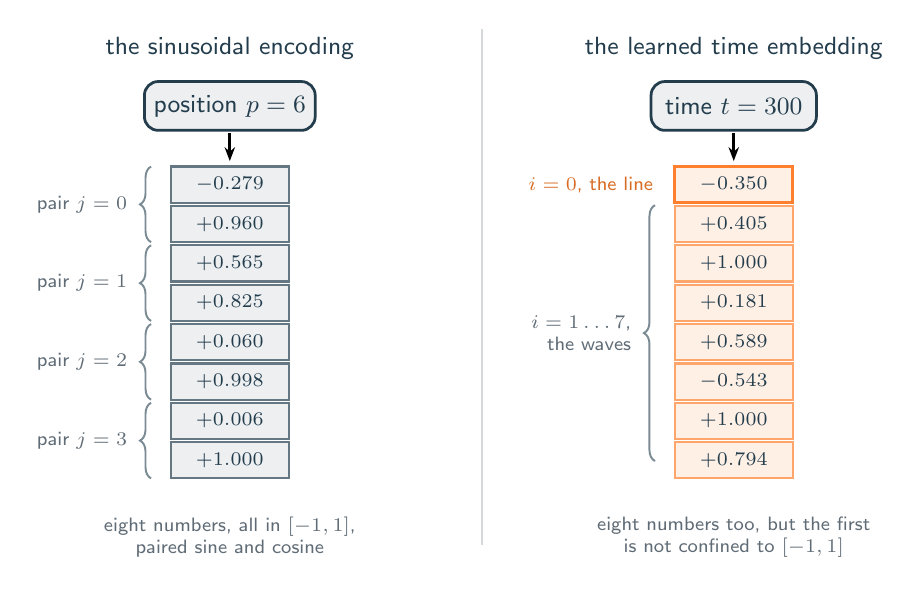
\begin{tikzpicture}[
    every node/.style={font=\sffamily},
    lab/.style={font=\sffamily\scriptsize, text=labelcolor},
    tag/.style={font=\sffamily\scriptsize, text=c2},
    hot/.style={font=\sffamily\scriptsize, text=c3!85!black},
    inp/.style={rectangle, rounded corners=5pt, draw=c2, fill=c2!8, text=c2,
                line width=1.0pt, minimum width=2.1cm, minimum height=0.62cm,
                font=\sffamily\small},
    cellL/.style={rectangle, draw=c2!70, fill=c2!8, line width=0.8pt,
                  minimum width=1.5cm, minimum height=0.46cm,
                  font=\sffamily\scriptsize, text=c2, inner sep=1pt},
    cellR/.style={rectangle, draw=c3!70, fill=c3!12, line width=0.8pt,
                  minimum width=1.5cm, minimum height=0.46cm,
                  font=\sffamily\scriptsize, text=c2, inner sep=1pt},
    arr/.style={-{Stealth[length=5pt]}, line width=1.0pt, color=c1},
]

\draw[c2!20, line width=0.8pt] (6.20, 0.05) -- (6.20, 6.60);

% ================================================================ left
\node[tag, font=\sffamily\small] at (3.00, 6.35) {the sinusoidal encoding};
\node[inp] (pin) at (3.00, 5.62) {position $p = 6$};
\draw[arr] (3.00, 5.28) -- (3.00, 4.92);

\foreach \k/\v in {0/{$-0.279$}, 1/{$+0.960$}, 2/{$+0.565$}, 3/{$+0.825$},
                   4/{$+0.060$}, 5/{$+0.998$}, 6/{$+0.006$}, 7/{$+1.000$}}{
    \node[cellL] at (3.00, {4.62 - \k*0.50}) {\v};
}
\foreach \j/\y in {0/4.37, 1/3.37, 2/2.37, 3/1.37}{
    \draw[decorate, decoration={brace, amplitude=4pt, mirror}, c2!60, line width=0.7pt]
        (2.00, {\y+0.48}) -- (2.00, {\y-0.48});
    \node[lab, anchor=east] at (1.82, \y) {pair $j = \j$};
}
\node[lab, anchor=north, align=center] at (3.00, 0.52)
    {eight numbers, all in $[-1, 1]$,\\ paired sine and cosine};

% ================================================================ right
\node[tag, font=\sffamily\small] at (9.40, 6.35) {the learned time embedding};
\node[inp] (tin) at (9.40, 5.62) {time $t = 300$};
\draw[arr] (9.40, 5.28) -- (9.40, 4.92);

\node[cellR, draw=c3, line width=1.2pt] at (9.40, 4.62) {$-0.350$};
\foreach \k/\v in {1/{$+0.405$}, 2/{$+1.000$}, 3/{$+0.181$}, 4/{$+0.589$},
                   5/{$-0.543$}, 6/{$+1.000$}, 7/{$+0.794$}}{
    \node[cellR] at (9.40, {4.62 - \k*0.50}) {\v};
}
\node[hot, anchor=east] at (8.50, 4.62) {$i = 0$, the line};
\draw[decorate, decoration={brace, amplitude=4pt, mirror}, c2!60, line width=0.7pt]
    (8.40, 4.36) -- (8.40, 1.11);
\node[lab, anchor=east, align=right] at (8.22, 2.73) {$i = 1 \dots 7$,\\ the waves};

\node[lab, anchor=north, align=center] at (9.40, 0.52)
    {eight numbers too, but the first\\ is not confined to $[-1, 1]$};

\end{tikzpicture}
\end{document}
